\documentclass[tikz,border=3mm,multi=tikzpicture]{standalone}
\usepackage[utf8]{inputenc}
\usepackage[T1]{fontenc}
\usepackage{helvet}
\renewcommand{\familydefault}{\sfdefault}
\usepackage{tikz}
\usetikzlibrary{angles,quotes,calc,intersections}
\begin{document}

\tikzset{every node/.append style={font=\sffamily\small}}
% TikZ 1
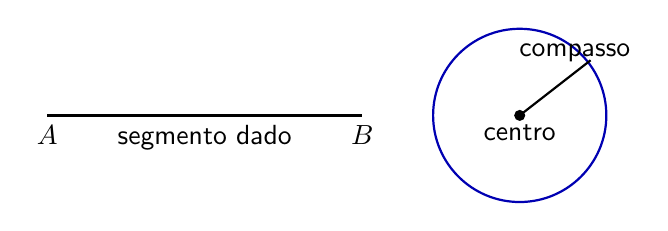
\begin{tikzpicture}[scale=1]
\coordinate (A) at (0,0); \coordinate (B) at (4,0);
\draw[thick] (A)--(B);
\node[below] at (A) {$A$}; \node[below] at (B) {$B$};
\node[below] at (2,0) {segmento dado};
\draw[blue!70!black,thick] (6,0) circle (1.1);
\draw[thick] (6,0)--(6.9,.7);
\fill (6,0) circle (2pt);
\node[below] at (6,0) {centro};
\node[above] at (6.7,.55) {compasso};
\end{tikzpicture}
% TikZ 2
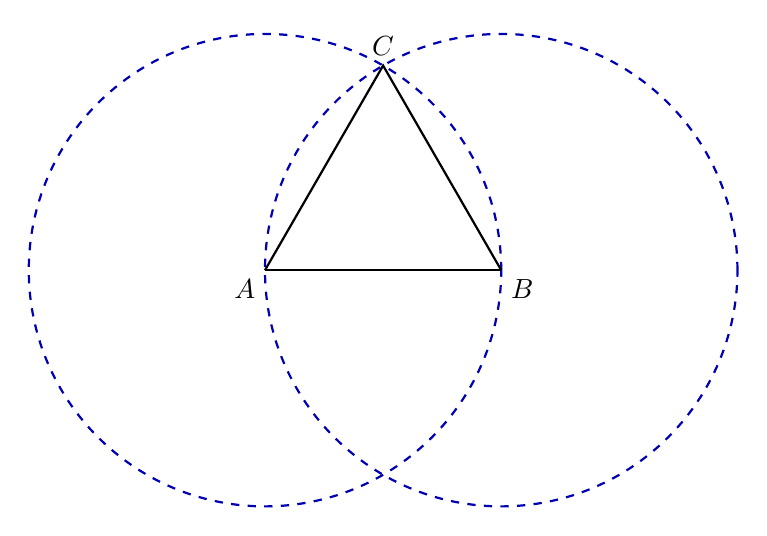
\begin{tikzpicture}[scale=1]
\coordinate (A) at (0,0); \coordinate (B) at (3,0); \coordinate (C) at (1.5,2.598);
\draw[thick] (A)--(B);
\draw[blue!70!black,thick,dashed] (A) circle (3);
\draw[blue!70!black,thick,dashed] (B) circle (3);
\draw[thick] (A)--(C)--(B);
\foreach \p/\pos in {A/below left,B/below right,C/above}{\node[\pos] at (\p) {$\p$};}
\end{tikzpicture}


% TikZ 3
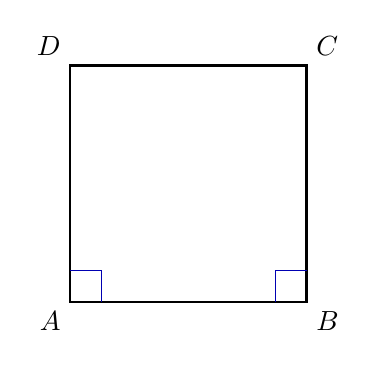
\begin{tikzpicture}[scale=1]
\coordinate (A) at (0,0); \coordinate (B) at (3,0); \coordinate (C) at (3,3); \coordinate (D) at (0,3);
\draw[thick] (A)--(B);
\draw[blue!70!black,thick,dashed] (A)--(D);
\draw[blue!70!black,thick,dashed] (B)--(C);
\draw[thick] (A)--(B)--(C)--(D)--cycle;
\pic[draw=blue!70!black, angle radius=4mm] {right angle=D--A--B};
\pic[draw=blue!70!black, angle radius=4mm] {right angle=A--B--C};
\foreach \p/\pos in {A/below left,B/below right,C/above right,D/above left}{\node[\pos] at (\p) {$\p$};}
\end{tikzpicture}
% TikZ 4
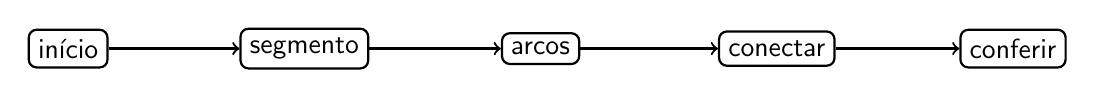
\begin{tikzpicture}[scale=1]
\node[draw,thick,rounded corners=1mm] (I) at (0,0) {início};
\node[draw,thick,rounded corners=1mm] (S) at (3,0) {segmento};
\node[draw,thick,rounded corners=1mm] (A) at (6,0) {arcos};
\node[draw,thick,rounded corners=1mm] (C) at (9,0) {conectar};
\node[draw,thick,rounded corners=1mm] (F) at (12,0) {conferir};
\draw[->,thick] (I)--(S);
\draw[->,thick] (S)--(A);
\draw[->,thick] (A)--(C);
\draw[->,thick] (C)--(F);
\end{tikzpicture}


% TikZ 5
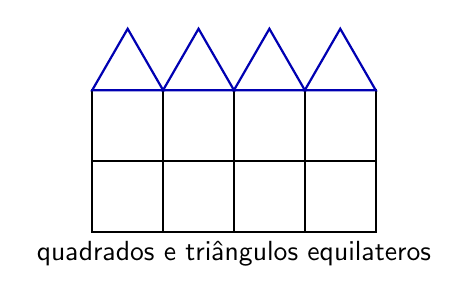
\begin{tikzpicture}[scale=.9]
\foreach \x in {0,1,2,3}{
  \foreach \y in {0,1}{
    \draw[thick] (\x,\y) rectangle +(1,1);
  }
}
\foreach \x in {0,1,2,3}{
  \draw[thick,blue!70!black] (\x,2)--(\x+.5,2.866)--(\x+1,2)--cycle;
}
\node[below] at (2,0) {quadrados e triângulos equilateros};
\end{tikzpicture}
\end{document}
